% Unit circle
% Author: Supreme Aryal
% A unit circle with cosine and sine values for some
% common angles.
\documentclass[12pt, a4paper]{article}
\usepackage{tikz}
\usepackage{verbatim}
\usetikzlibrary{calc}
\usetikzlibrary{arrows,shapes}

\usepackage[top=1in,bottom=1in,right=1in,left=1in]{geometry}
\begin{document}

\noindent\makebox[\textwidth]{
\begin{minipage}{2\textwidth}
\begin{center}
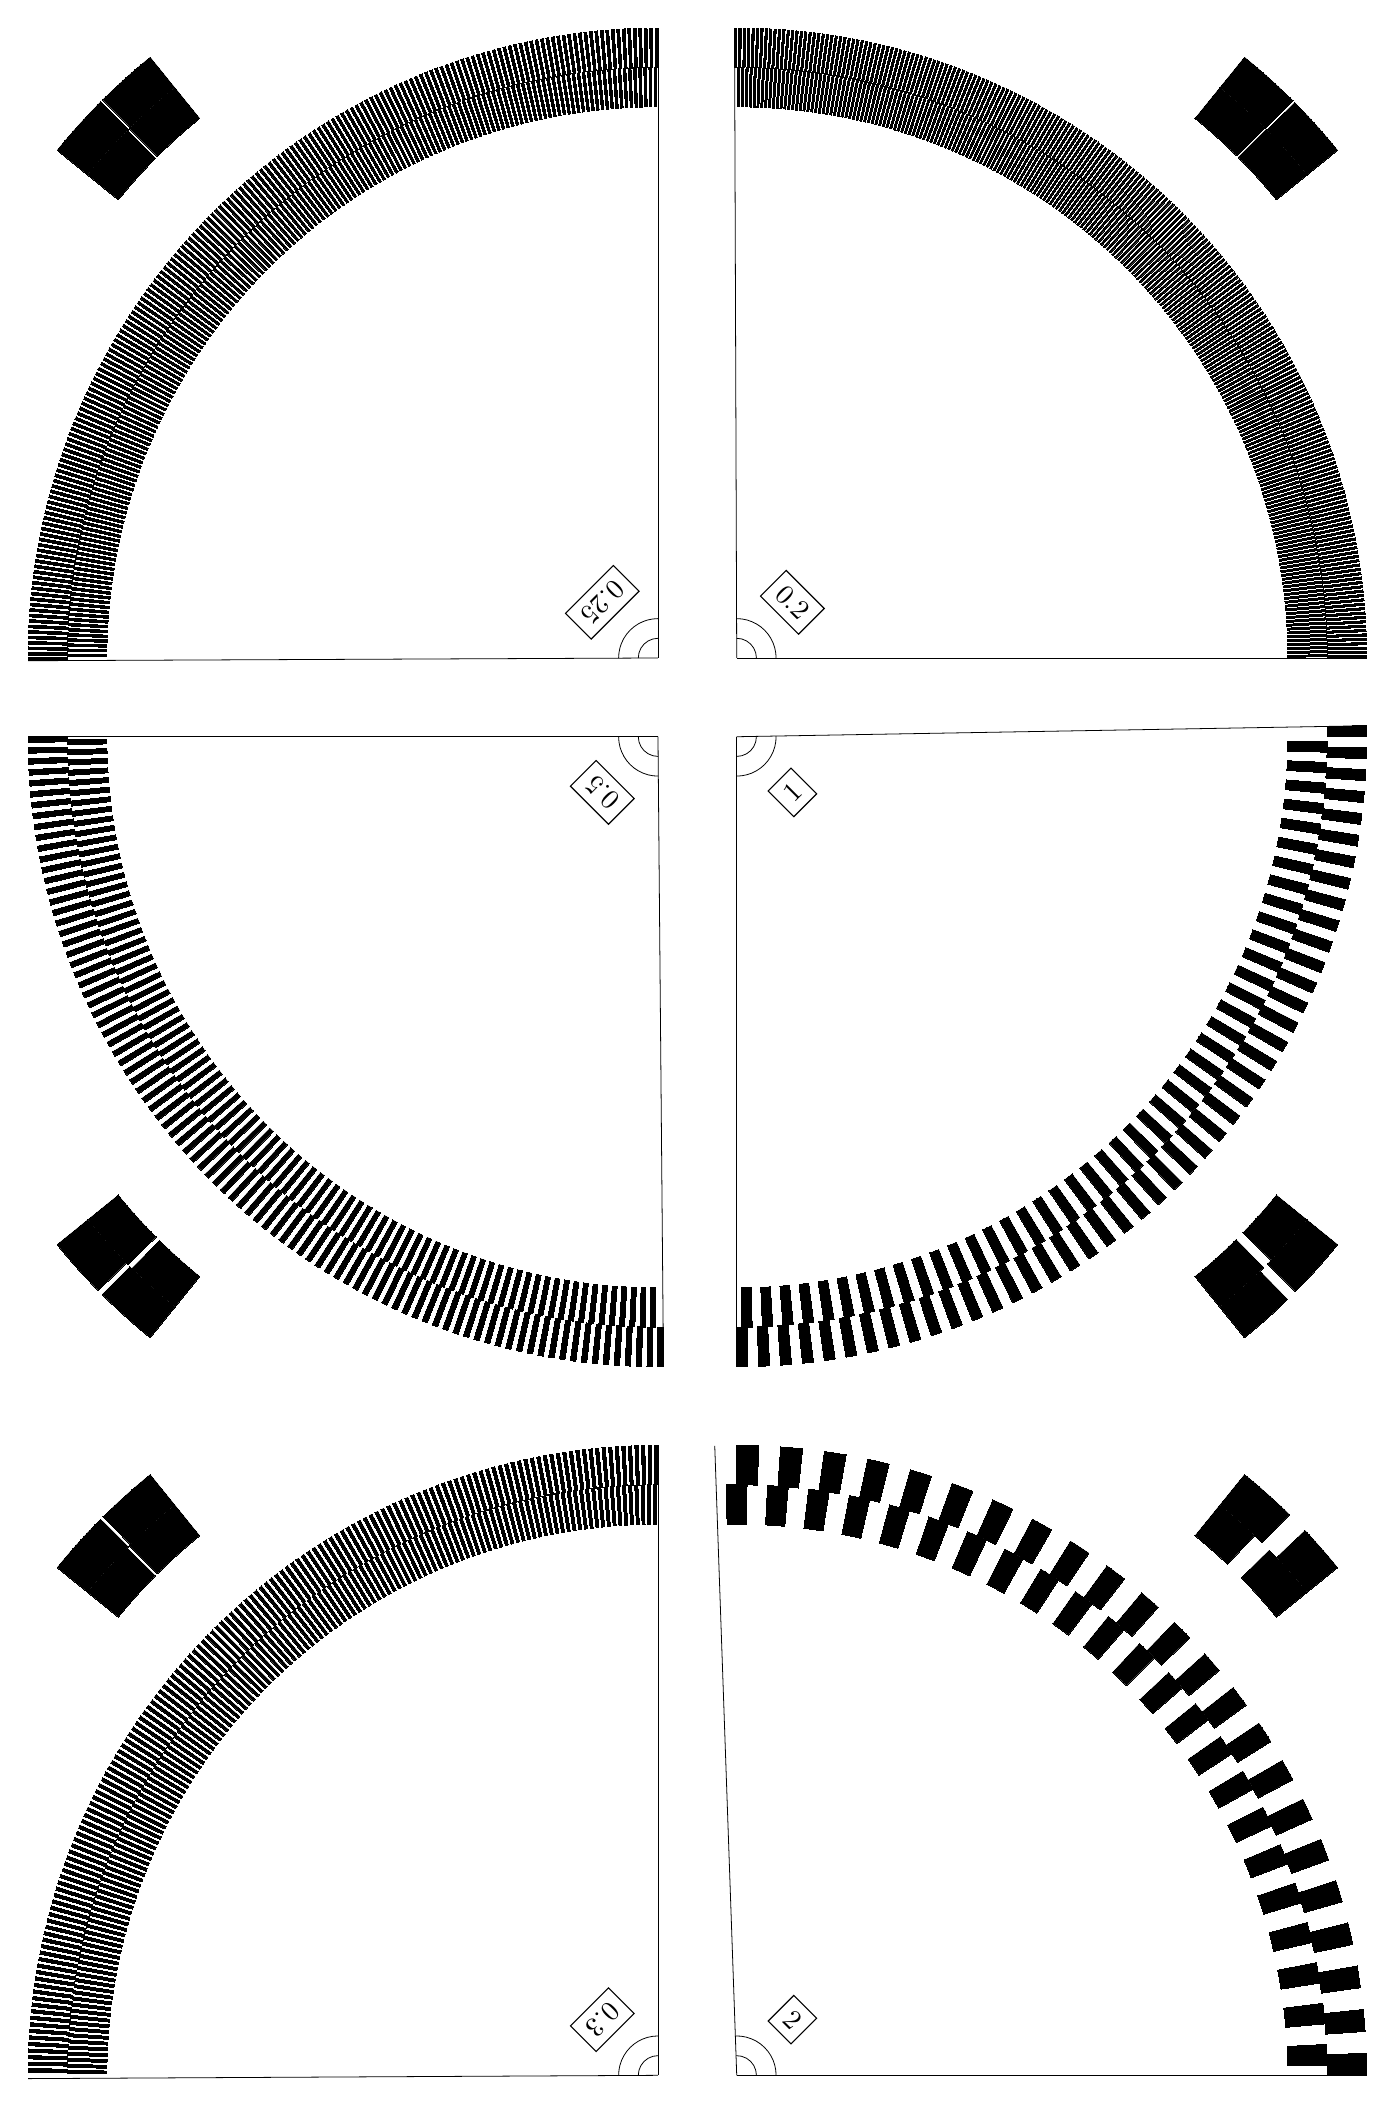
\begin{tikzpicture}

\newcommand{\drawArc}[4]{%Angle1,Angle2,Radius1,Radius2
    	\draw[fill=black, line width=0mm]
	(#2:#3) arc
	(#2:#1:#3) --
	(#1:#4) arc
	(#1:#2:#4) --
	cycle;
}

\newcommand{\rotaryEncoderLines}[5]{
   \pgfmathsetmacro{\angleSecond}{#1+#3*2};
    \foreach \a in {#1,\angleSecond,...,#2}
  {
	\drawArc{\a}{\a+#3}{#4}{#5};
  }
}
\newcommand{\rotaryEncoder}[5]{
	\rotaryEncoderLines{#1}{#2}{#3}{#4-#5}{#4};
	\pgfmathsetmacro{\angleAtwo}{#1+#3/2};
	\rotaryEncoderLines{\angleAtwo}{#2}{#3}{#4-#5*2}{#4-#5};

	\draw[line width=0.1mm] (0,0) -- (#1:#4);
  	\draw[line width=0.1mm] (0,0) -- (#2+#3:#4);
  	\draw[line width=0.1mm] (#1:2.5mm) arc (#1:#2+#3:2.5mm);
  	\draw[line width=0.1mm] (#1:5mm) arc (#1:#2+#3:5mm);

	\pgfmathsetmacro{\angleMid}{(#1+#2)/2};
	\node[draw,rotate=-\angleMid] (t) at (\angleMid:10mm) {#3};
\begin{scope}[shift={(\angleMid:#5*4)}]
	\pgfmathsetmacro{\widthMask}{6};
	\drawArc{\angleMid+#3*3/4}{\angleMid+\widthMask}{#4-#5*2}{#4-#5}; %inner left
	\drawArc{\angleMid-#3/4}{\angleMid-\widthMask}{#4-#5*2}{#4-#5}; %inner right
	\drawArc{\angleMid+#3/4}{\angleMid+\widthMask}{#4-#5}{#4}; %outer left
	\drawArc{\angleMid-#3*3/4}{\angleMid-\widthMask}{#4-#5}{#4}; %outer right
\end{scope}
}
\begin{scope}[]
	\rotaryEncoder{0}{90}{0.2}{80mm}{5mm}
\end{scope}
\begin{scope}[shift={(-1cm,0cm)}]
	\rotaryEncoder{90}{180}{0.25}{80mm}{5mm}
\end{scope}
\begin{scope}[shift={(-1cm,-1cm)}]
	\rotaryEncoder{180}{270}{0.5}{80mm}{5mm}
\end{scope}
\begin{scope}[shift={(0cm,-1cm)}]
	\rotaryEncoder{270}{360}{1}{80mm}{5mm}
\end{scope}
\begin{scope}[shift={(0cm,-18cm)}]
	\rotaryEncoder{0}{90}{2}{80mm}{5mm}
\end{scope}
\begin{scope}[shift={(-1cm,-18cm)}]
	\rotaryEncoder{90}{180}{0.3}{80mm}{5mm}
\end{scope}
    \end{tikzpicture}
\end{center}
\end{minipage}
}
\end{document}
